\chapter{Regression}

Regression is a form of supervised machine learning with as goal to take continuous data and find the equation that best fits the data. This way you'll be able to forecast a specific value.

\section{Linear Regression}
The best fit function searched is just a linear line. See figure \ref{fig:linearregression} for an example. Since linear regression is the basis of almost all machine learning algorithms (it is also used in Neural Networks for example), we will elaborate a bit more on how it actually works. \\
\\
As we know a first order line can be simply represented as $y = mx + b$. We know $x$ since it are our labels and when training we also know $y$ since it are our features (which we know, since it's supervised learning). So the goal of linear regression is to calculate $m$ and $b$, calculating $m$ is achieved with the following formula: $m = \dfrac{\overline{x}\cdot\overline{y}-\overline{xy}}{(\overline{x})^2-\overline{x^2}}$ where the bar over the letters signifies a mean or average. To calculate $b$ the following formaly can be used: $b = \overline{y} - m\overline{x}$. When you use these formulas to calculate the regression line you are actually minimising the sqaured error between the regression line's y values and the data's y values. To know how well the regression line predicts the data's y values you can check the outcome of the \emph{r squared method}, see chapter \ref{chap:general_terms}.

\begin{figure}
\centering
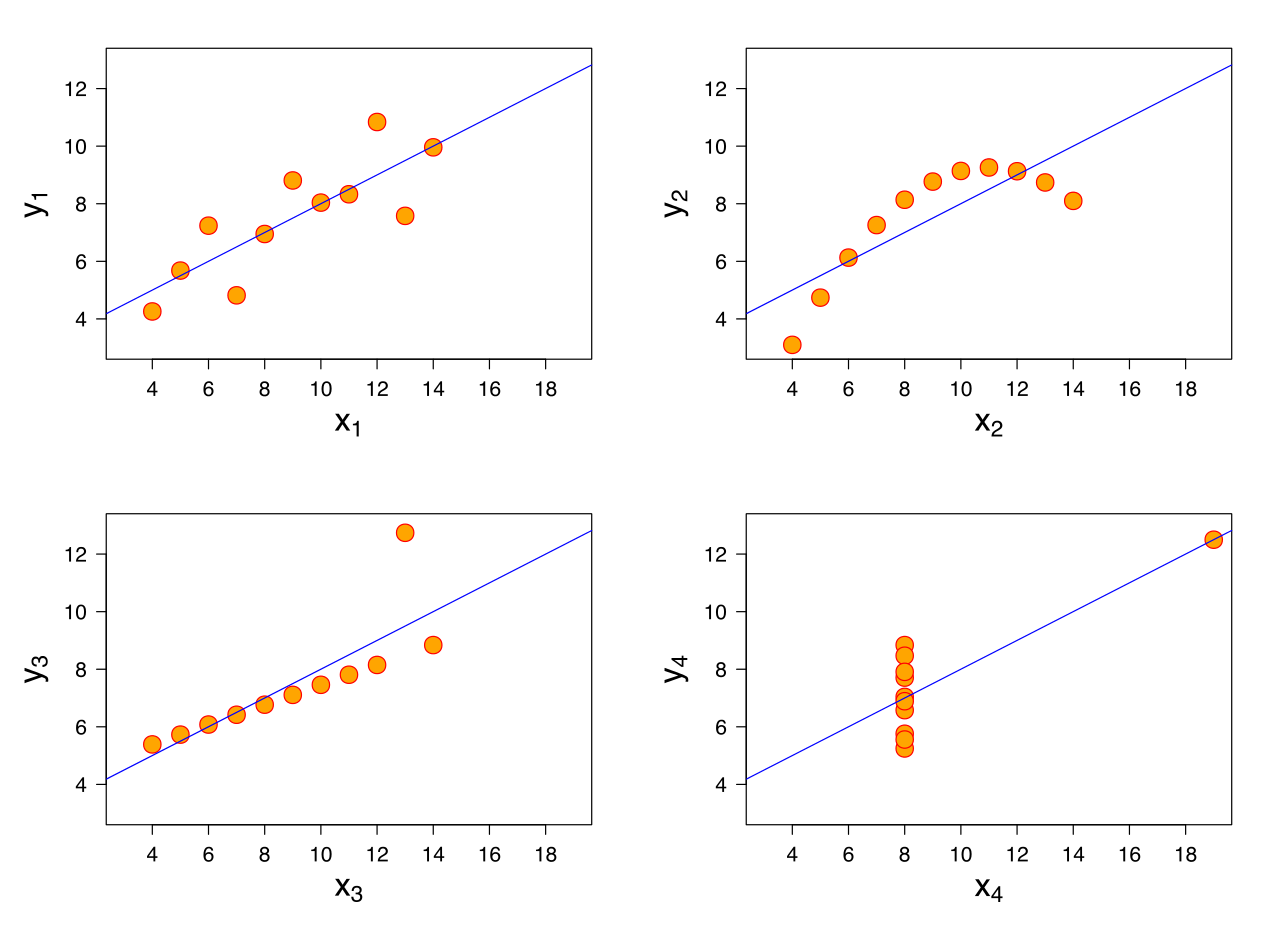
\includegraphics[width=1\textwidth]{images/linear_regression.png}
\caption{\label{fig:linearregression}Four examples of the function found by linear regression based on the given data points.}
\end{figure}

\subsection{Code examples}
Two code approaches have been made. The first approach uses the \emph{sklearn} kit for doing linear regression as well as experimenting with some support vector machines, the approach can be found in appendix \ref{code:regression}. The second approach shows a more basic linear regression which illustrates it's fundamentals. Since linear regression is the basis of a lot of machine learning algorithms, this code can help you understand the basic building blocks of all these machine learning alorithms. It also shows how the \emph{r squared method} works. This code can be found in appendix \ref{code:manualregression}.
